% !TeX encoding = UTF-8
% !TeX program = xelatex
% ----------------------------------------------------------------------------------------------------------------
% Appel des packages de base
% ----------------------------------------------------------------------------------------------------------------
\documentclass[10pt,a4paper]{report}
\usepackage{styles/preambule_college}
\usepackage{styles/preambule_personnalisation}


\setcounter{secnumdepth}{3}



%\definecolor{darkblue}{rgb}{0.12,0.47,0.87}
%
%\titleformat{\chapter}[display] 
%	{\fontsize{17pt}{12pt}\selectfont \bfseries}
%	{\textcolor{darkblue}{\chaptertitlename\ \thechapter: #1}}
%	{20pt}
%	{\Huge}
%
%\titleformat{name=\chapter,numberless}[display] 
%	{\fontsize{17pt}{12pt}\selectfont \bfseries}
%	{\textcolor{darkblue}{#1}}
%	{20pt}
%	{\Huge}

% ----------------------------------------------------------------------------------------------------------------
% Début du document
% ----------------------------------------------------------------------------------------------------------------
\begin{document}





\chapterFormat




\chapter*{Environnement de travail}

Le collège met à disposition des étudiants et des professeurs divers outils informatiques. Pour être efficient dans son travail, il est nécessaire d'en connaître l'existence et l'usage\dots





\section{Infrastructure du collège}



\subsection{Machines et réseau}

Des ordinateurs fixes sont à disposition à la bibliothèque, dans les salles de classes et dans les salles informatiques. Les photocopieurs peuvent être utilisés comme imprimante réseau depuis les postes fixes. Le WiFi est disponible dans tout l'établissement.

Ces infrastructures sont dédiées au travail. Cela veut dire que tout ce qui passe sur le réseau fait l'objet d'une surveillance. Cela permet à l'établissement de déterminer au besoin qui a utilisé l'infrastructure à mauvais escient et de prendre les mesures correspondantes.



\subsection{Identifiant}

Chaque étudiant ou professeur doit se connecter avec son identifiant (nom d'utilisateur et mot de passe) pour accéder à l'infrastructure informatique. Le nom d'utilisateur est public ou peut être deviné par n'importe qui. Le mot de passe est personnel et doit le rester.

\attention Tout activité effectuée par un utilisateur identifié sur le réseau est de la responsabilité de la personne qui a défini le mot de passe correspondant. C'est de la responsabilité de chaque utilisateur de changer de mot de passe suffisamment souvent pour éviter les soucis.

\exemple*{
	Alice a eu accès au mot de passe de Bob, peut-être parce que Bob le lui a donné, ou parce qu'il l'avait écrit dans un endroit accessible. Peut-être aussi parce que le mot de passe était facile à deviner ou parce que Bob utilise tout le temps le même depuis des années ou encore parce qu'il en a qu'un seul pour différents services (ses comptes Instagram, Tik Tok, Snapchat\dots). Peut-être aussi Bob s'est-il montré naïf en remplissant un faux questionnaire l'incitant à changer son mot de passe ou en répondant à un faux appel téléphonique\footnote{Il s'agit de \emphdef{phishing} appelé aussi \emphdef{hameçonnage}}\dots \ Dans tous les cas, Alice peut se connecter à l'infrastructure en se faisant passer pour Bob, faire ce qu'elle veut et ce sera à Bob d'assumer ce qu'elle fait !
}

\remarque*{
	Au passage, Alice a comis quelques infractions, non seulement contre le règlement du collège et la charte informatique, mais aussi contre le droit suisse. Le Code pénal ne punit pas encore l'usurpation d'identité en tant que telle, mais une modification de l'art. 179 devrait bientôt le permettre. Dans tous les cas, selon ce qu'a fait Alice après s'être connectée, elle pourrait être accusée de s'être introduite sur un système informatique sans en avoir le droit (art. 143), d'avoir calomnié ou diffamé Bob, de l'avoir escroqué d'avoir utilisé frauduleusement un ordinateur\dots \ Ce sont des infractions qui peuvent conduire à des amendes voire à de la prison.
}





\newpage





\subsection{Services en ligne}

L'identifiant personnel donne accès non seulement aux machines du collège, mais aussi aux services en ligne suivants.



\subsubsection{creusets.net}

Le site web du collège ne sert pas uniquement à télécharger la liste de classe lors de la dernière semaine des vacances ! Il permet de trouver toutes les informations pratiques et, uniquement pour les personnes connectées, d'accéder à des téléchargements particuliers ou à des galeries de photo.

\begin{figure}[H]
	\centering
	\href{https://creusets.net}{
		
\includegraphics[width=0.75\linewidth]{images/capture_creusets_20210811.png}
	}
	\caption{\protect \href{https://edu.vs.ch}{Site web du collège}}
	\label{fig:capturecreusets20210811}
\end{figure}

Le site est accessible à l'adresse \href{https://creusets.net}{https://creusets.net}.



\subsubsection{Plateforme d'apprentissage : Moodle}

Moodle est un système de gestion de contenu ou \emphdef{Content Management System} (CMS) en anglais. Moodle est un CMS dédié à l'enseignement. Il s'agit d'un logiciel libre développé depuis une vingtaine d'années et utilisé par plusieurs centaines de milliers de sites Web dans plus de 200 pays. Toutes les grandes universités l'utilisent, en particulier en Suisse.

\begin{figure}[H]
	\centering
	\href{https://moodle-lcc.edu-ictvs.ch/}{
		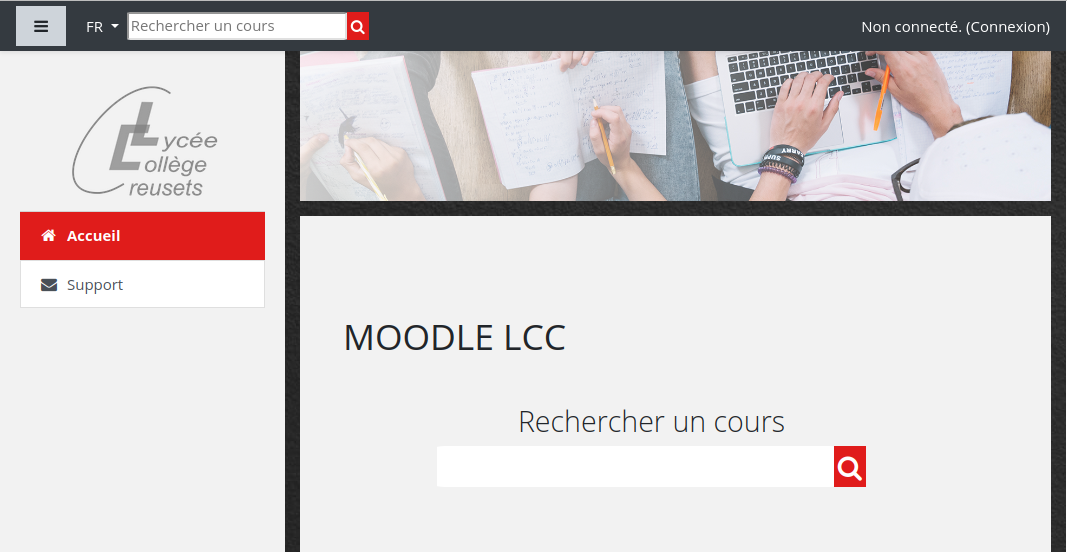
\includegraphics[width=.75\linewidth]{images/capture_moodle_lcc_20210811}
	}
	\caption{\protect\href{https://moodle-lcc.edu-ictvs.ch/}{Moodle LCC}}
	\label{fig:capturemoodlelcc20210811}
\end{figure}

Le Moodle LCC est accessible à l'adresse suivante : \href{https://moodle-lcc.edu-ictvs.ch/}{https://moodle-lcc.edu-ictvs.ch}

\encadre[Les logiciels libres]{
	Il existe plusieurs définition d'un \emphdef{logiciel libre} (voir par exemple \autocite{LogicielLibre2021}). Toute reprennent cependant les bases posées par la \href{https://www.gnu.org/philosophy/free-sw.html}{Free Software Foundation} (FSF). Ce type de logiciel garantit que "les utilisateurs ont la liberté d'exécuter, copier, distribuer, étudier, modifier et améliorer ces logiciels" \autocite{DefinitionLogicielLibre}. N'importe quel programmeur (vous dans quelques mois peut-être) peut donc voir comment est fait le logiciel pour en comprendre le fonctionnement détaillé. Cela peut servir à vérifier qu'il ne s'y cache rien de malveillant, de corriger des bugs ou de proposer de nouvelles fonctionnalités.\\[1ex]
	La plupart du temps, ces logiciels sont d'ailleurs gratuits, même si gratuité n'est pas synonyme de liberté. Selon la FSF :
	\enquote{\textelp{} “free software” is a matter of liberty, not price. To understand the concept, you should think of “free” as in “free speech,” not as in “free beer”.} \autocite{WhatFreeSoftware}.\\[1ex]
	La \emphdef{licence} d'une logiciel est ce qui détermine ce qu'on a le droit de faire avec. Les principales licences libres sont les \href{https://fr.wikipedia.org/wiki/Licence_publique_g\%C3\%A9n\%C3\%A9rale_GNU}{GNU} \autocite{LicencePubliqueGenerale2021}, \href{https://fr.wikipedia.org/wiki/Licence_BSD}{BSD} \autocite{LicenceBSD2021} ou \href{https://fr.wikipedia.org/wiki/Licence_Apache}{Apache} \autocite{LicenceApache2021}.
}



\subsubsection{ENT}

Le canton du Valais met à disposition une plateforme nommée ENT pour "environnement numérique de travail". Il s'agit d'un produit commercial de Microsoft.

\begin{figure}[H]
	\centering
	\href{https://edu.vs.ch}{
		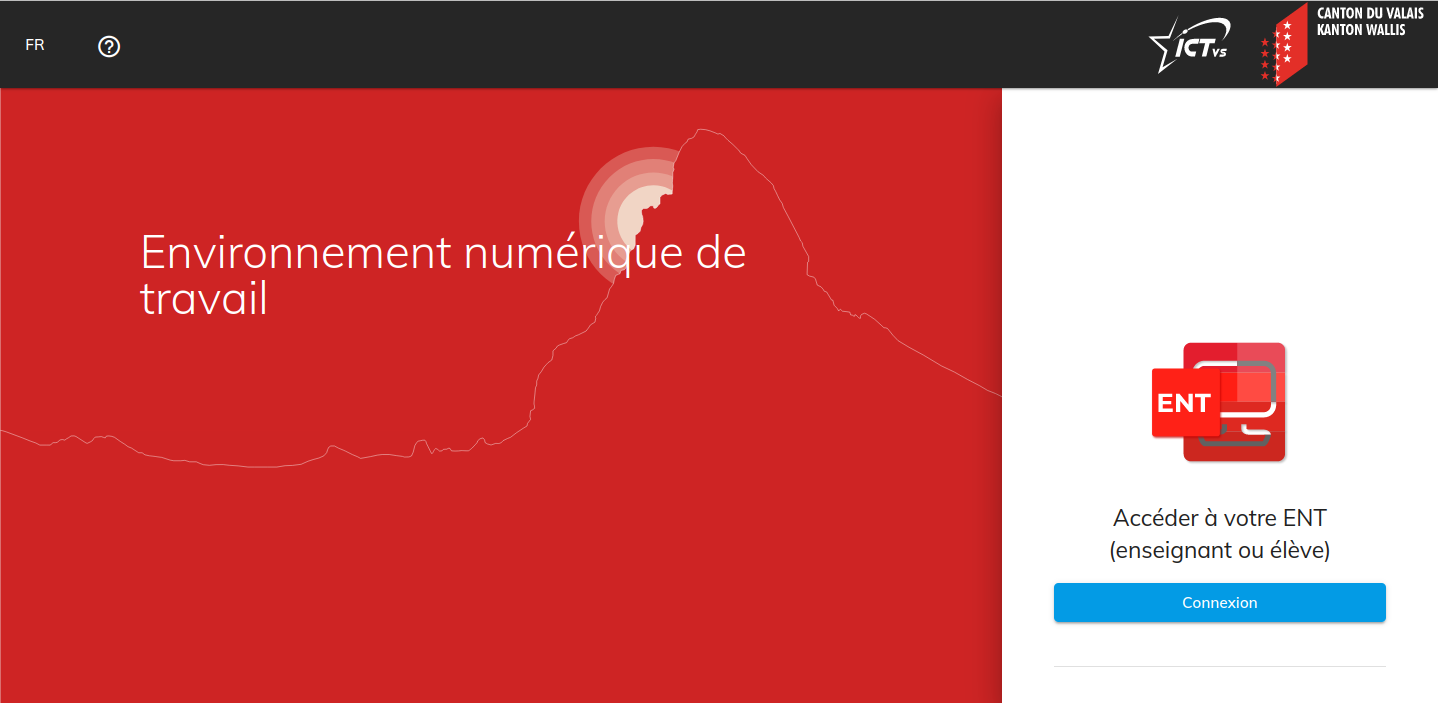
\includegraphics[width=0.75\linewidth]{images/capture_ENT_20210811.png}
	}
	\caption{\protect \href{https://edu.vs.ch}{ENT -- Environnement numérique de travail}}
	\label{fig:captureent20210811}
\end{figure}

L'accès à l'ENT se fait à l'adresse \href{https://edu.vs.ch}{https://edu.vs.ch}.

La page principale présente les divers produits sous forme de tuiles.

\begin{figure}[H]
	\centering
	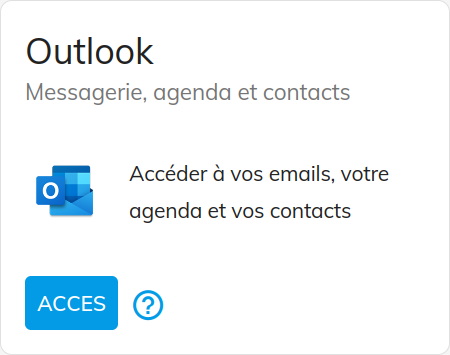
\includegraphics[width=0.18\linewidth]{images/capture_ENT_tuile_outlook_20210811}
	\hfill
	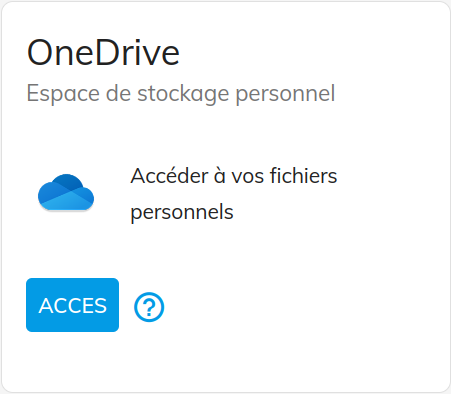
\includegraphics[width=0.18\linewidth]{images/capture_ENT_tuile_OneDrive_20210811}
	\hfill
	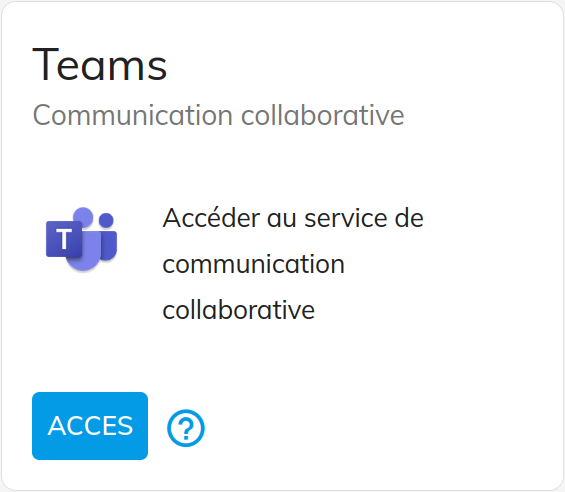
\includegraphics[width=0.18\linewidth]{images/capture_ENT_tuile_Teams_20210811}
	\hfill
	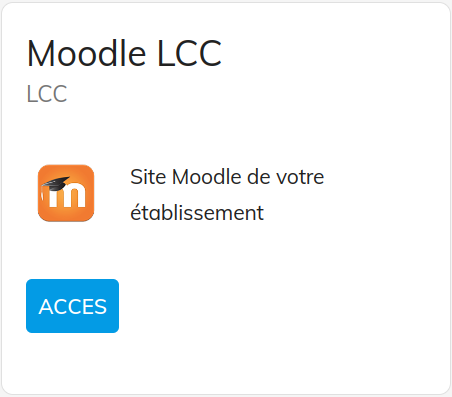
\includegraphics[width=0.18\linewidth]{images/capture_ENT_tuile_moodle_20210811}
	\caption{Tuiles des fonctions principales de l'ENT}
	\label{fig:tuilesENT}
\end{figure}

\begin{description}
	\item[Outlook] Ce terme regroupe deux choses distinctes :
		\begin{itemize}
			\item un service d'e-mails avec les contacts et les agenda;
			\item des logiciels permettant de se connecter au service e-mail. Il en existe des versions pour téléphone mobile (sous Android ou iOS), pour ordinateurs Apple sous OS X et pour ordinateurs Windows.
		\end{itemize}
		Il est possible d'accéder aux service de messagerie sans application Outlook, simplement depuis la tuile présente dans l'ENT. On parle alors de \emphdef{webmail} puisqu'il s'agit d'utiliser un service e-mail depuis son navigateur web. \\
		Il est aussi recommandé d'installer une application de messagerie sur son ordinateur et son téléphone pour accéder plus directement à ses e-mails. A noter que sur Android, Apple (iOS ou OS X), Windows ou Linux, il existe des applications préinstallées qui permettent de se connecter à son e-mails sans avoir à installer l'application Outlook.
	\item[OneDrive] un espace de stockage pour y déposer des fichiers.
	\item[Teams] Il s'agit d'un logiciel de visioconférence et de travail collaboratif. Pour faire une visioconférence, il faut évidemment que l'ordinateur dispose d'une caméra et d'un micro, ce qui n'est pas le cas des ordinateurs des salles de classe et de la bibliothèque.
	\item[Moodle] Lien vers le Moodle LCC depuis l'ENT (voir ci-dessus).
\end{description}

\remarque*{
	Pour toute question concernant l'ENT, commencez par aller lire les informations (normalement réservées aux prof\dots) sur \href{https://support.ictvs.ch/index.php/fr/}{https://support.ictvs.ch/index.php/fr/}
}

\encadre[Les logiciels propriétaires]{
	Les logiciels propriétaires sont le contraire des logiciels libres. La plupart des logiciels commerciaux sont de ce type. Ainsi, une entreprise garde le secret sur la manière dont est faite son logiciel. Il est donc impossible de savoir comme il fonctionne réellement et encore moins de le modifier. \\[1ex]
	Le \emphdef{reverse engineering} ou \emphdef{rétro-ingéniérie} est un procédé permettant d'étudier un logiciel pour en comprendre le comportement lorsqu'on ne peut pas savoir comment il a été conçu. Cette pratique est illégale la plupart du temps\dots
}







\section{Bases de l'utilisation}



\subsection{Vocabulaire}

Cette section donne quelques brèves définition. La plupart de ces notions seront étudiées plus en détail durant le cours d'informatique.

\begin{itemize}
	\item Un \emphdef{ordinateur} ou \emphdef{computer} est un système de traitement automatique de l'information basé sur le principe d'une machine de Turing (voir \autocite{MachineTuring2021}). Il n'y a pas que les postes de travail qui correspondent à cette définition : les \emphdef{ordinateurs personnels} ou \emphdef{personal computers} (PC), les tablettes, les smartphones, les machines des centres de calcul ont tous la même structure. \\
		Un ordinateur est composé d'une partie \emphdef{matérielle} et d'une partie \emphdef{logicielle.}
	\item Le \emphdef{matériel} informatique est l'ensemble des composants éléctriques, électroniques, mécaniques qui composent un ordinateur. On les sépare habituellement en :
		\begin{itemize}
			\item \emphdef{composants} : les parties formant le corps de la machine et comprenant notamment le boîtier, l'alimentation, la carte-mère qui relie et alimentent autres composants, les unités de calcul, les unités de mémoire, les cartes spécialisées (carte son, vidéo\dots)
			\item \emphdef{les périphériques} : les parties venant se connecter au corps de la machine, répartis entre les périphériques d'entrée (clavier, souris, scanner, caméra, micro\dots), les périphériques de sortie (écran, haut-parleurs, imprimantes\dots), les périphériques d'entrée-sortie (mémoire externe, cartes WiFi, smartphones\dots)
		\end{itemize}
		Cette classification est assez souple. Par exemple, une interface WiFi peut très bien être un composant ou un périphérique, un téléphone peut être un périphérique d'entrée uniquement (quand on récupère des photos) ou un périphérique d'entrée-sortie (lorsqu'on l'utilise comme modem pour accéder à Internet).
\end{itemize}

\encadre[Alan Turing]{
	Alan Mathison Turing (voir \autocite{AlanTuring2021}) est une star de l'informatique. Dans les années 1930-1950, ses travaux, souvent parfaitement théoriques, ont permis de créer les premiers ordinateurs. Par exemple, ce qu'on appelle \emphdef{machine de turing}, est une modèle théorique de ce que devrait faire une personne ou une machine pour exécuter une procédure. Il ne s'agit donc pas d'un objet, mais de mathématiques ! Sans ce modèle, pas d'ordinateur\dots \\[1ex]
	Turing est célèbre pour avoir contribué à décrypter les messages codés que s'échangeaient les allemand à l'aide de leurs machines Enigma (voir \autocite{EnigmaMachine2021}). Ceci a contribué a réduire significativement la durée de la deuxième guerre mondiale. \\[1ex]
	Turing a aussi travaillé sur les ébauches de l'intelligence artificielle (IA). Son fameux \emphdef{test de Turing} \autocite{TestTuring2021} est toujours mentionné lorsqu'il faut déterminer si une machine est réellement intelligente. Turing propose l'expérience suivante : des personnes sont appelées à dialoguer des machines. Si au bout de la discussion, il ne leur est pas possible de dire si leur interlocuteur était une machine ou une personne, la machine est dite intelligente. Un petit essai avec Eliza \autocite{ElizaTherapeuteElectronique} ? N.B. Lorsqu'un informaticien vous dit que vous venez d'échouer au test de Turing, ce n'est pas un compliment\dots \\[1ex]
	Malgré l'ampleur de sa contribution, la Grande-Bretagne ne fit pas de cadeau à Turing et le condamna en 1952 pour son homosexualité.\\[1ex]
	Turing meurt en 1954, empoisonné au cyanure, une pomme croquée à côté de lui. Plusieurs rumeurs sont associées à son décès : Turing aurait ingéré le poison en croquant une pomme empoisonnée, comme dans le dessin animé de Blanche-Neige et les Sept Nains qu'il appréciait réellement. Il l'aurait fait suite à la dépression que causa sa condamnation. Et ceci aurait donné l'idée du logo Apple. Pour les spécialistes de la vie de Turing, ces histoires, bien qu'intéressantes, ne correspondent pas à la réalité\dots.
}

\begin{itemize}
	\item Un \emphdef{logiciel}, ou aussi \emphdef{programme}, \emphdef{application}, \emphdef{app}, \emphdef{software}, \emphdef{soft}, est une série d'instruction que l'on fait exécuter à une machine sur une série de données.
		\begin{enumerate}
			\item Le \emphdef{système d'exploitation} ou \emphdef{operating system} (OS) est un ensemble de logiciel qui sert à gérer le matériel. L'OS est responsable de faire démarrer la machine, de gérer les composants et les périphériques. Il doit fournir une interface aux programmes utilisateurs pour que ces derniers n'aient pas à se soucier des détails matériels de la machine sur laquelle ils tournent.\\[1ex]
			Il existe des OS pour tout : les PC (Windows, OS X, Linux, BSD), les téléphones (Android, iOS), les objets connectés (mynewt, snappy, TinyOS)\dots
			\item Les \emphdef{logiciels utilisateur} interagissent avec l'OS pour exécuter toutes sortes d'activités (lire une vidéo, rédiger un document, lancer une recherche web, piloter une machine\dots). Ce sont les logiciels avec lesquels vous interagissez le plus.
		\end{enumerate}
	\item Un \emphdef{fichier} est la manière usuelle de stocker nos informations sur un ordinateur. Le fichier regroupe les informations contenant un document particulier. Il est stocké physiquement sur une mémoire permanente (qui ne n'efface pas quand on éteint l'ordinateur) comme un disque dur, un SSD, une clé USB\dots
	\item Les \emphdef{répertoires}, ou \emphdef{dossiers}, \emphdef{classeurs}, \emphdef{directories}, sont des fichiers particuliers : ils contiennent une liste de fichiers. Ils servent à ordonner les fichiers de manière à s'y retrouver plus rapidement ou à séparer des données destinées à différents usages (p. ex. les fichiers des applications et celles de l'utilisateur). Habituellement, un répertoire est présenté à l'utilisateur comme une sorte de boîte dans laquelle on peut mettre des fichiers et d'autres répertoires. \\[1ex]
		Lorsqu'on place un répertoire à l'intérieur d'un répertoire, on parle de \emphdef{sous-répertoire}.
\end{itemize}

\encadre[Utilité des répertoires]{
	Certains OS comme Android, iOS, voire OS X, masquent les répertoires et les fichiers. Ils proposent de retrouver les informations par des outils de recherche. Si cela est pratique sur un smartphone, ce n'est pas une stratégie que l'on peut utiliser quand on travaille de manière professionnelle sur un ordinateur. Utilisez des répertoires ! \\[1ex]
	Dans tous les cas, vos ordinateurs utilisent des répertoires standardisés :
	\begin{itemize}
		\item Windows : Users ou 
		\item Mac
	\end{itemize}
}

\encadre[Nommer fichiers et répertoires]{
	Même si on peut utiliser n'importe quel caractère pour définir des noms de fichiers, l'usage des espaces et des signes diacritiques (accents, cédilles\dots) finit tôt ou tard par créer des prblèmes, p. ex. lors du transfert des fichiers, de leur archivage ou pire, de leur restauration après qu'on les ait perdus. \\[1ex]
	Pour les noms un peu long, il existe deux conventions typographiques :
	\begin{description}
		\item[\emphdef{\emphdef{snake case}}] : nom\_un\_peu\_long (en utlisant le caractère de soulignement);
		\item[\emphdef{camel case}] : nomUnPeuLong (en utilisant les majuscules).
	\end{description}
}

\begin{itemize}
	\item Le \emphdef{type de fichier} ou \emphdef{format de fichier} est la manière dont une application enregistre les informations. Un logiciel de dessin ne stocke pas les données de la même manière qu'un logiciel de musique. Beaucoup d'applications ont leurs propres types de fichiers, mais il existe aussi de nombreux types de fichiers standardisés qui peuvent être utilisés par différentes applications (p. ex. les documents pdf).
	\item L'\emphdef{extension de fichier} est un suffixe au nom du fichier qui permet à l'OS de savoir quelle application utiliser pour traiter un fichier. Elle est indiquée par un point suivi habituellement de trois, voire quatre lettres. Voir ci-dessous l'encadre contenant les extensions les plus courantes. \\[1ex]
		Par exemple, un appareil photo produit généralement des fichiers au format Joint Photographic Experts Group et le nomme automatiquement en comptant le nombre de photos qu'il a prise. Ainsi la photo 1024 aura le nom P1024.jpg ou P1024.jpeg. Lorsqu'on double clique sur ce fichier, le ".jpg" indiquera au système d'aller chercher une application qui gère ce format. \\[1ex]
		Habituellement on nomme le type de fichier par son extension et on parle ainsi de fichiers jpg, pdf, docx, html\dots \\[1ex]
		\attention Modifier l'extension du fichier le rend illisible : l'ordinateur va essayer de l'ouvrir avec le mauvais programme. Pour \emphdef{convertir} un fichier d'un format à un autre, il faut passer par une application qui connaît les deux formats. \\[1ex]
		\attention Il faut parfois modifier les préférences de son OS pour qu'il affiche les extensions de fichiers. C'est généralement une bonne chose à faire\dots
	\item L'\emphdef{arborescence} est une structure informatique qu'on peut représenter par un arbre, avec un point de départ, des branches et des sous-branches, mais pas de cycle. Lorsqu'on place des fichiers et des répertoires dans d'autres répertoires, on créé l'\emphdef{arborescence des fichiers}.
	\item La \emphdef{racine} ou \emphdef{base} de l'arborescence est le niveau le plus bas de la structure, p. ex. c:\textbackslash \ sous Windows ou simplement / sur Mac ou Linux.
	\item Le \emphdef{chemin d'accès} est la liste des répertoires et sous-répertoires qu'il faut suivre depuis la racine pour arriver au fichier recherché. Par exemple si un fichier document.txt se trouve dans le répertoire "travail" de l'utilisatrice Sara son chemin d'accès sera vraisemblablement c:\textbackslash Users \textbackslash Sara \textbackslash travail \textbackslash document.txt sous Windows ou /home/sara/travail/document.txt sous Mac ou Linux.
\end{itemize}

\encadre[Extensions de fichiers courantes]{
	Pour être efficient sur un ordinateur, il faut connaître quelques extensions de fichiers courantes et le type de fichier s'y rapportant.
	\begin{description}
		\item[pdf] documents non modifiables, prévus pour être imprimés tel quel. Leur faible taille les rends facilement transmissibles sur les réseaux.
		\item[png, jpg, bmp] fichiers d'\emphdef{images raster}. Ils contiennent une trame de pixels. Ces \emphdef{pixels}, un raccourci de \textit{picture elements}, sont des carrés suffisamment petits pour n'être pas visible à moins de zoomer dessus.
		\item[svg] fichiers d'\emphdef{images vectorielles}, contenant la description géométrique de l'image (des arcs de cercle, des segments, des polygones\dots). On peut zoomer tant qu'on veut, l'ordinateur recalcule à chaque fois l'image et elle reste parfaitement nette.
		\item[mp3, wav, aa, flac, ogg] fichier audio.
		\item[mpg, avi, mov, mp4, wmv] fichier vidéo.
		\item[doc, xls, ppt] fichiers de Microsoft Office pour Word, Excel et PowerPoint
		\item[odt, ods, odp] fichiers de LibreOffice et associés pour Writer, Calc et Impress
		\item[html] fichiers contenant une page web
		\item[csv, txt] fichiers ne contenant que du texte, sans aucune mise en forme. Le csv est l'abbréviation de Comma-separated Values. C'est un format très courant pour échanger des données entre des logiciels.
		\item[zip, 7z, bz2, tar, rar] fichiers compressés. Ces fichiers contiennent un autre fichier, voire un répertoire complet mais dont la taille a été réduite. Cela permet de gagner du temps pour transmettre des documents ou d'encapsuler des répertoires en vue de les transmettre en une fois (p. ex. pour faire une pièce jointe pour un e-mail) ou pour les archiver.
	\end{description}
	Il en existe bien d'autres, par exemple sur la \href{https://fr.wikipedia.org/wiki/Liste_d\%27extensions_de_fichiers}{liste de Wikipédia} \autocite{ListeExtensionsFichiers2021}.
}

\begin{itemize}
	\item Un \emphdef{serveur} est un ordinateur ou un logiciel ayant un fonctionnement particulier : il passe son temps à attendre que quelqu'un lui transmet une demande. Par exemple, un serveur web attend qu'on lui demande une page web. Il y a de nombreux types de services et donc de serveurs qui s'occupent par exemple de pages web, d'e-mails, de configurations, d'identifiants\dots 
	\item Un \emphdef{client} est un ordinateur ou un logiciel qui interroge un serveur.
	\item Le \emphdef{cloud} ou \emphdef{nuage} désigne Internet (cela fait référence à la représentation habituelle d'Internet dans les schémas de réseaux). Le \emphdef{cloud computing} ou \emphdef{informatique en nuage} fait référence à une architecture informatique. Toutes sortes de fonctionnalités peuvent être accédées à distance par Internet, par exemple
		\begin{description}
			\item[stockage de fichiers] comme Dropbox, Nextcloud, Google Drive, Amazon S3, Microsoft OneDrive\dots \ Ces services permettent de stocker ces fichiers quelque part sur Internet. On ne sait pas où, mais il y a quelque part un data center qui a un ordinateur muni d'un disque dur qui contient vos données. Avec Nextcloud, un logiciel libre, on peut faire ça chez soi sur ses propres machines.
			\item[applications] comme Collabora ou Onlyoffice, basés sur LibreOffice, Office 365 en ligne, Google Docs, Etherpad, Scratch online et toutes sortes d'autres applications qu'on peut accéder directement depuis un navigateur.
			\item[distribution de vidéo] comme Mediacast, youtube, vimeo, PeerTube\dots
			\item[centres de calcul] comme AWS Lambda. Cela permet d'accéder à une grande puissance de calcul au besoin.
			\item[hebergement] pour faire fonctionner des serveurs entiers à distance (serveurs web, e-mail\dots)
		\end{description}
	\item \emphdef{Synchroniser} des fichiers consiste à comparer des copies d'un même fichier situées à deux endroits différents et à faire en sorte que toute modification d'une des copies soit reportée sur les autres copies. C'est le cas par exemple avec OneDrive ou Nextcloud : les fichiers situés sur votre ordinateur personnel, votre téléphone ou votre tablette\dots \ sont toujours les mêmes : toute modification à un endroit est reportée partout. \\[1ex]
		Il est clair que si vous modifiez les copies d'un même fichier, en même temps, sur deux machines différentes, il n'est plus possible de les synchroniser sans votre intervention.
	\item le \emphdef{backup} ou \emphdef{sauvegarde} consiste à faire une copie de secours. Cette copie est utilisée principalement lorsque les données originales sont perdues ou dégradées. \\[1ex]
		\attention Il ne faut pas confondre synchronisation et sauvegarde : si on endommage un fichier, le système de synchronisation va propager le problème partout et le fichier original est perdu. \\[1ex]
		Lorsqu'on fait sérieusement des sauvegardes, on prévoit de faire des copies à des intervalles de temps réguliers (chaque heure, jour, semaine\dots) selon les besoins, et on stocke les copies dans des lieux sécurisés. Par exemple une copie hebdomadaire est gardée dans une armoire fermée au bureau et une copie est amenée chaque mois dans un coffre à la banque, voire est envoyée sur un autre continent !
	\item \emphdef{Automatique} : peut être utiliser pour dire tout et n'importe quoi. Méfiez-vous en et faites préciser !
	\item \emphdef{Sécurité} : de même.
\end{itemize}



\subsection{Traitement de texte}

Le traitement de texte est un sujet d'étude en soi et ne fait pas partie de ce cours. Une seule remarque : lorsqu'on met en forme un texte, par exemple avec Writer ou Word, il est \emph{nécessaire} d'utiliser les styles.

Si vous ne le faites pas habituellement ou si vous ne savez pas ce que c'est, trouvez-vous un tutoriel le plus rapidement possible !



\subsection{Utilisation du mail}

Chaque membre de l'établissement a une adresse prenom.nom@edu.vs.ch. Il s'agit d'un moyen de communication professionnel et il convient de l'utiliser comme tel. En particulier, un e-mail correctement rédigé :
\begin{itemize}
	\item comporte l'adresse du destinataire (sans cela votre e-mail n'ira pas bien loin);
	\item le sujet qui précise le contenu du mail (ce champ est visible lorsque les e-mails sont présentés sous forme de liste et aide s'y retrouver);
	\item une formule d'annonce en début de courrier (Madame, Monsieur\dots);
	\item une formule de salutation à la fin (au minimum "Meilleures salutations");
	\item une signature (votre prénom, votre nom et éventuellement votre classe).
\end{itemize}

Un e-mail professionnel doit être rédigé en utilisant un registre de langage soutenu et en évitant les familiarités, les abréviations et les émoticônes.

Les e-mails sont gérés par un \emphdef{serveur mail}, ici un serveur Microsoft Exchange. Pour accéder à vos e-mails, vous pouvez le faire à l'aide de votre navigateur. On parle alors de \emphdef{webmail}. Cependant, lorsqu'on a plusieurs adresses personnelles et professionnelles, il devient très pratique d'utiliser un application dédiée (le \emphdef{client mail}), par exemple Thunderbird (libre et disponible sur tous les OS), mail par défaut sur Mac et Outlook par défaut sur Windows.




\subsection{Sauvegardes}

Il est de la responsabilité de chacun de sauvegarder ses fichiers (documents de travail, photos, vidéos, messages\dots). Multiplier les copies dans des fichiers différents, des répertoires différents, sur des clés USB ou des disques externes est une mauvaise stratégie : 
\begin{itemize}
	\item On finit rapidement par ne plus savoir quelle est la bonne version.
	\item Si les sauvegardes sont sur le même appareil que les données, une panne fait perdre à la fois les fichiers et leurs sauvegardes.
	\item Les clés USB ne sont pas des dispositifs très fiables : elles tombent facilement en panne, si on ne les a pas perdues avant\dots
	\item Si votre sauvegarde est sur un équipement connecté en permanence à votre ordinateur, une attaque par ransomware vous détruira les copies et les sauvegardes en même-temps.
\end{itemize}

Le plus simple est de trouver un logiciel de sauvegarde dans lequel on peut configurer les fichiers à sauvegarder et l'intervalle de temps entre les sauvegardes. Ces logiciels gèrent sont suffisamment bien fait pour ne copier que ce qui a été modifié depuis la dernière sauvegarde et permet de retrouver l'entier de ces fichiers en cas de panne. Les copies de sauvegardes doivent être faites sur une dispositif externe à son ordinateur qui est éteint ou débranché entre chaque sauvegardes. On peut aussi envisager de mettre de temps en temps une copie de sauvegarde ailleurs qu'à la maison.



\subsection{Transférer des fichiers}

Il existe diverses solutions pour transférer des fichiers à quelqu'un d'autre, voire à soi-même :
\begin{enumerate}
	\item placer le fichier dans un répertoire partagé ou synchronisé;
	\item envoyer un lien permettant de télécharger le fichier;
	\item copier le fichier sur un support amovible (clé USB, disque externe, carte SD\dots).
\end{enumerate}

Généralement, le mail n'est pas un bon moyen de transférer des fichiers. Généralement la taille et le type des fichiers que l'on peut envoyer sont restreints. Par ailleurs, si on doit envoyer le contenu de tout un répertoire, il faut ajouter à la main chaque fichier, ce qui peut être assez long.

Une manière de contourner le problème est de créer un fichier compressé (ou zippé) du répertoire et d'essayer de le placer en pièce jointe (si sa taille et son type sont acceptés\dots).



\subsection{Gestion des mots de passe}

La création et la gestion des mots de passe peut vite devenir pénible. Un bon mot de passe doit être à la fois difficile à trouver, suffisamment long (plus de 10-12 caractères) et doit souvent répondre à des règles précises (comporter au moins une majuscule, une minuscule, un caractère spécial, un chiffre\dots). 

Par ailleurs, un mot de passe ne doit être utilisé que pour une seule application. Par exemple, votre mot de passe professionnel doit être réservé à ça. Votre mot de passe Tik Tok doit être différent de celui pour Whatsapp et ne doivent pas être les mêmes que celui de votre mail personnel\dots

Et en plus, il faut s'en rappeler ! Même quand on a dans les deux cents mots de passe !

La meilleure manière de s'en tirer est d'utiliser un gestionnaire de mots de passe. C'est comme un coffre-fort à clés : on place toutes ses clés dans une armoire blindée et ensuite \dots \ on la ferme avec une autre clé ! L'avantage est qu'on besoin que d'une seule clé, celle de l'armoire. Évidemment, pour que ça fonctionne, il faut que l'armoire soit très solide et que sa serrure soit de très bonne qualité.

Avec un gestionnaire de mot de passe, c'est exactement pareil. On va placer les mots de passe dans un fichier encrypté. L'encryptage fait office de coffre-fort et sa serrure est le seul mot de passe dont il faut se rappeler. Evidemment, si on perd ce dernier mot de passe\dots

Par ailleurs, un mot de passe permet de remplir sans intervention les champs "nom d'utilisateur" et "mot de passe" dès qu'il détecte un site web qu'il connaît. A l'usage, on se connecte une seule fois à son gestionnaire et ensuite, il fait tout le boulot pour nous : il génère des mots de passe très forts, il les enregistre, il les écrits pour nous dans les sites web.

\href{https://bitwarden.com/}{bitwarden}

Bitwarden est un gestionnaire libre, sûr, gratuit pour un usage privé et s'intègre aussi bien à son navigateur web qu'à son téléphone ou sa tablette. Son usage est conseillé dès qu'on a plus d'une dizaine de mot de passe et devient indispensable quand on en a plusieurs centaines.





\section{Raccourcis claviers}

Pour éviter de passer des heures et des heures sur son ordinateur, il faut maîtriser le clavier\dots

\remarque*{
	Il vaut largement la peine de perdre du temps pour apprendre à taper à dix doigt et à l'aveugle. Vu le temps qu'un étudiant au collège, puis à l'université passe sur un clavier, c'est un investissement des plus rentables ! \\
	Il existe des méthodes commerciales très efficaces, comme \href{https://www.taptouche.com/fr/}{Tap'Touch} ou d'autres gratuites comme \href{https://www.typing.com/}{typing.com/}.
}

Par ailleurs, la plupart des actions courantes et fréquentes peuvent être exécutées à l'aide de raccourcis clavier, ce qui permet de gagner aussi passablement de temps lorsqu'on travaille. Voici une liste de raccourcis qui sont valables dans presque tous les logiciels. Il en existe bien d'autres et il se peut que ces raccourcis aient été modifiés dans des logiciels particulier, mais c'est peu fréquent. Il vaut donc la peine de connaître ces logiciels et il vaut encore mieux que ses doigts les connaissent tous seuls.

\remarques*{
	\listtopsep
	\begin{itemize}
		\item ctrl-c signifie appuyer aussi longtemps que l'on veut sur la touche contrôle (ctrl) du clavier et pendant qu'on appuie sur cette touche, appuyer une fois sur la touche c.
		\item Les raccourcis sont donnés ici avec la touche ctrl. Ceci est valable sur Windows, Linux et autres. Sur Mac, il faut remplacer ctrl par cmd (la touche commande).
	\end{itemize}
}

\begin{description}
	\item[ctrl-a] tout sélectionner
	\item[ctrl-c] copier
	\item[ctrl-v] coller
	\item[ctrl-x] couper
	\item[ctrl-s] enregistrer
	\item[ctrl-maj-s] enregistrer sous
	\item[ctrl-z] annuler la dernière opération
	\item[ctrl-f] rechercher
	\item[ctrl-o] ouvrir
	\item[ctrl-w] fermer
	\item[ctrl-q] quitter
\end{description}










\nocite{CreusetsNet,ENTEnvironnementNumerique,MoodleLCC}
\printbibliography[title=Notes bibliographiques,heading=subbibnumbered]





\end{document}
